\chapter{Einleitung}

Heutzutage spielen Daten eine immer wichtiger Rolle.
In vielen Firmen und Forschungseinrichtungen wächst die Zahl an unterschiedlichen Daten stetig.
Im \textit{Rethink Data Report 2020} \textcite{rethink_data_2020} wurde eine Studie durchgeführt, die eine Steigerung von 42\% der Menge an anfallenden Daten pro Jahr prognostiziert.
Diese Daten sind zum Beispiel durch den vermehrten Einsatz von IoT-Geräten oder ausführlicher werdende Analysen zurückzuführen.
Auch, dass es durch moderne Cloud-Speicher-Lösungen einfacher geworden ist große Datenmengen zu speichern, begünstigt diese Entwicklung.
Daten sind eine wertvolle Ressource und müssen entsprechend gut verwaltet werden.
Durch die unterschiedlichen Formate und Strukturen, zum Beispiel Datenbanktabellen, JSON-Datei oder Bilder ist die Verwaltung ein komplexes Thema.
Die Bewältigung der organisatorischen Aufgaben fällt in den Bereich Data Governance.
Diese Arbeit beschäftigt sich mit den technischen Herausforderungen Daten aus einer Vielzahl von Datenquellen zu verwalten.

In vielen Unternehmen besteht das Problem, dass Daten in sogenannten Datensilos gelagert werden.
Das bedeutet, dass für verschiedene Anwendungen oder Format isolierte Speichersysteme verwendet werden.
Dabei entsteht das Problem, dass der Überblick, welche Daten es in der gesamten Systemlandschaft gibt verloren geht.
Auch Daten, für Analysen, untereinander zu Verknüpfen wird mit zunehmender Datenmenge und Variation schwieriger.

Ein klassischer Ansatz, der die Analysen vereinfachen soll ist das Data Warehouse.
Ein Data Warehouse besteht aus verschiedenen Datamarts, in denen Daten für bestimmte Analysen abgelegt werden.
Daten werden aus den Quellsystemen geladen, mit verschiedenen Transformationen auf ein für den Datamart globales Schema gebracht und dann abgespeichert \parencite{dw}.
Dieses Vorgehen wird auch ETL (Extract Transform Load) genannt, da die Daten erst aus der Quelle extrahiert, dann transformiert und gespeichert werden und erst nach diesen Schritten für eine Analyse geladen werden können.
Bei der Transformation der Daten kann es oft passieren, dass ein Teil ihres Informationsgehalts verloren geht, da nicht alle Felder in den Datamart übernommen werden.
Außerdem wird eine Änderung an einem Schema teurer, je mehr Daten bereits integriert wurden.
Als Lösung für diese Problem wurden Data Lakes vorgeschlagen \parencite{dixon2010pentaho,datalake_03}.

\section{Data-Lake-Systeme}
\label{sec:einleitung-datalake}

Ein Data Lake ist ein System, das die Erfassung, Verfeinerung, Archivierung und Erkundung von Daten vereinfacht und verbessert \parencite{datalake_01}.
Es sollen große Datenmengen möglichst kostensparend speichern und verschiedenste Formate verarbeiten werden können \parencite{datalake_02}.
Diese System verfolgen dabei den ELT (Extract Load Transform) Ansatz.
Das Kernprinzip ist die Speicherung der Daten in ihrem Rohformat.
Die Transformation findet erst statt, nachdem die Daten für weitere Verarbeitungen geladen wurden.
Dadurch fällt der Aufwand für eine Transformation vor dem Speichern, wie bei einem Data Warehouse, weg und Daten sind schneller für weitere Verarbeitungen bereit.
Außerdem gehen dabei keine Informationen mehr verloren.

Ein Data-Lake-System basiert auf vier verschiedenen Ebenen, wie zum Beispiel in \cref{fig:datalake}.
Diese sind die Interaktion-, Transformations-, Speicher- und Ingestion-Ebene.
Über die Interaktions-Ebene kann auf die Daten im Data Lake zugegriffen und Metadaten verwaltet werden.
Die Transformations-Eben bereitet die Daten auf, nachdem diese aus der Speicher-Ebene geladen wurden.
Als letztes gibt es die Ingestion-Ebene.
Diese ist für die Integration von Daten in den Data Lake verantwortlich.
Gleichzeitig werden hier auch Metadaten aus den Daten extrahiert.
Die Umsetzung eines solchen Data  Lakes kann je nach Voraussetzungen des Einsatzbereichs variieren.

\begin{figure}
    \centering
    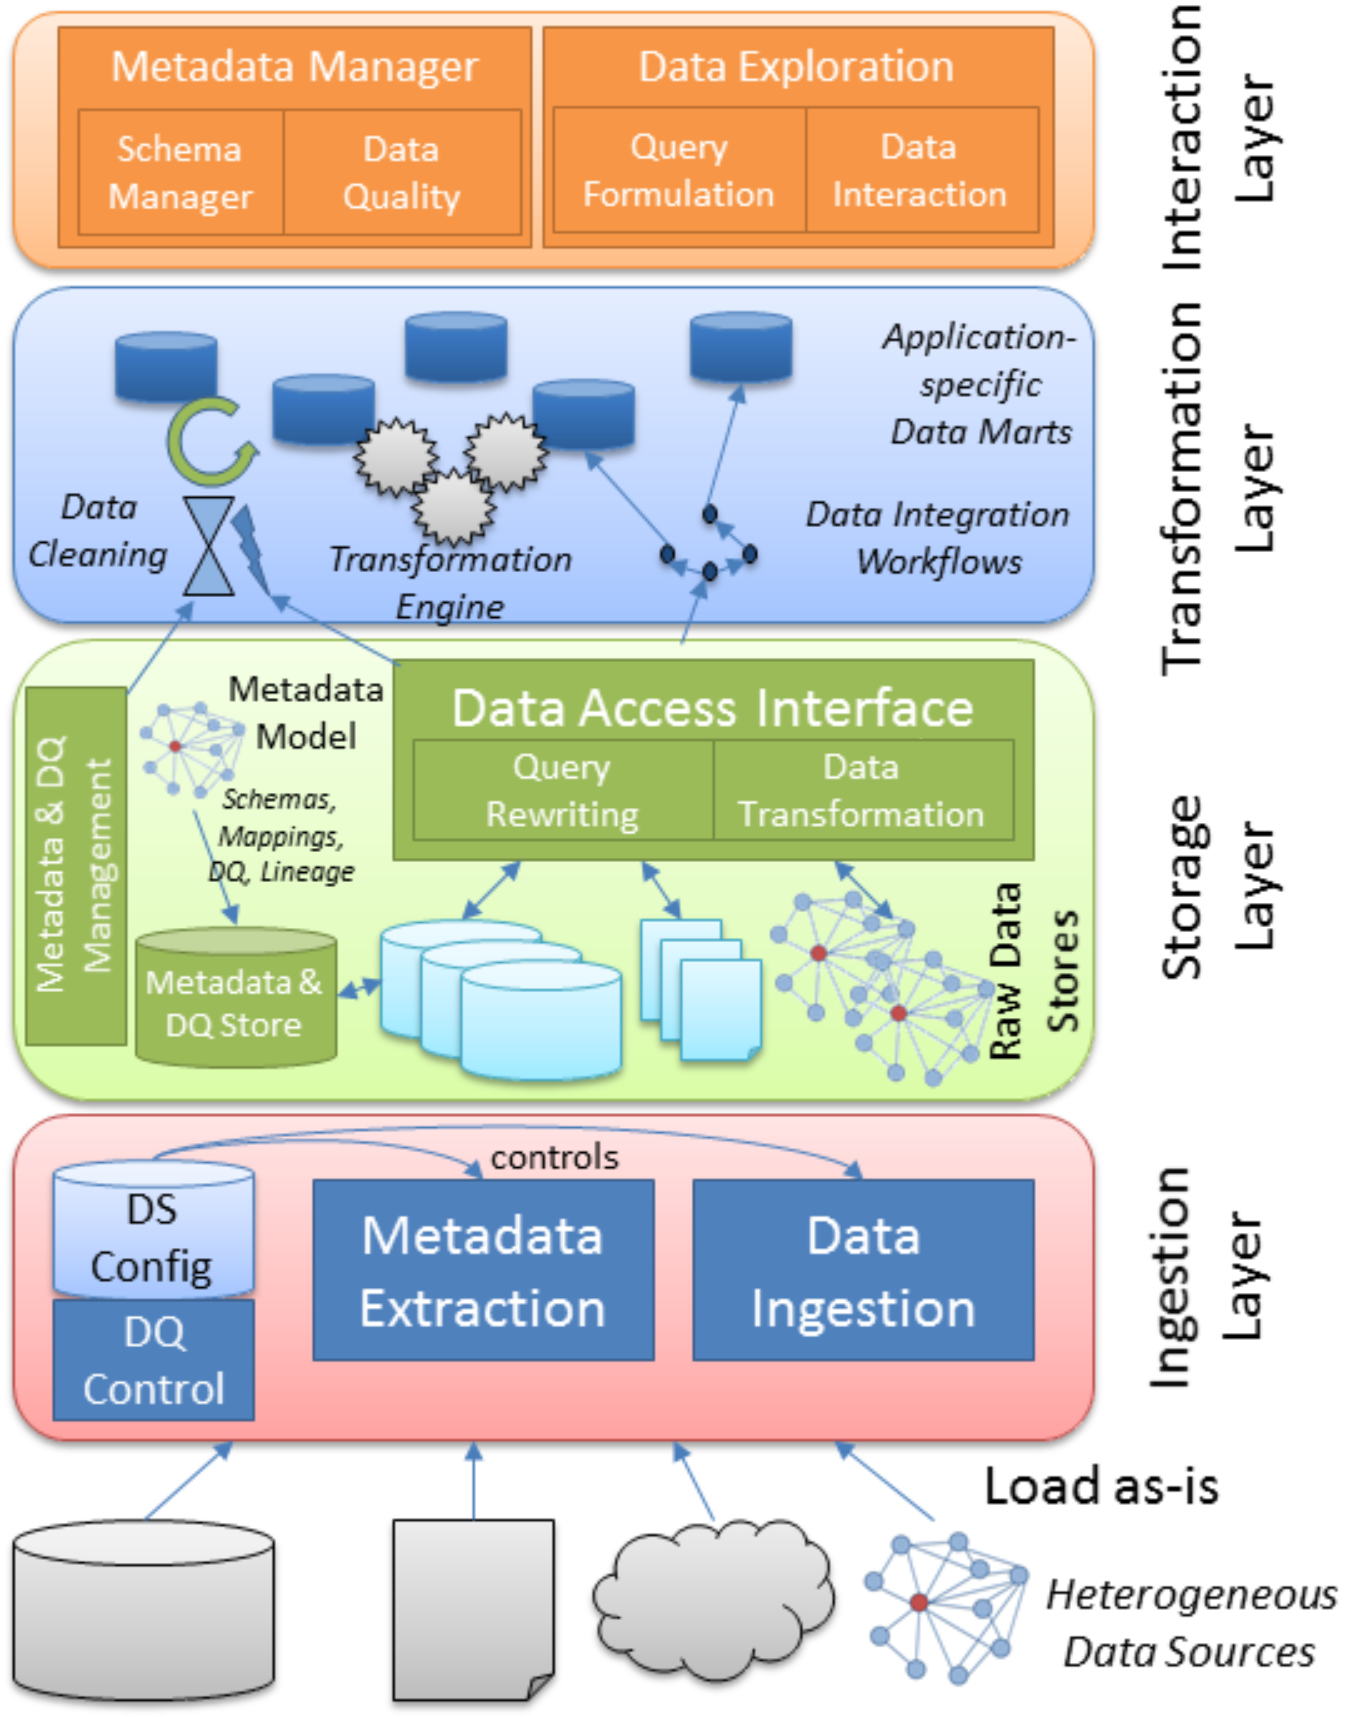
\includegraphics[width=.645\textwidth]{Grafiken/data_lake_architecture.PNG}
    \caption{Architektur eines Data Lakes \parencite{datalake_03}}
    \label{fig:datalake}
\end{figure}
\vfill

\pagebreak

\section{Motivation}
\label{sec:einleitung-motivation}

In einem Data Lake spielen die Metadaten eine zentrale Rolle.
Die Qualität der Metadaten bestimmt, wie gut Daten im Data Lake gefunden und in einen Zusammenhang gebracht werden können.
In den Metadaten können dabei sowohl Informationen über die Herkunft von Daten als auch über deren Inhalt oder Qualität stehen.

Für das HIT-Institut der Hochschule Niederrhein soll ein Data Lake entwickelt werden, der für die Verwaltung der Daten eingesetzt wird.
In diesem System sollen verschiedene Quellen zusammengebracht werden.
Dazu gehören Datenbank-Systeme, Dateien und Daten aus speziellen Software-Systemen, die über eine REST-API erreichbar sind.
Hier sollen die Daten jedoch nicht nur einmalig in das System geladen, sondern kontinuierlich aktualisiert werden.
Der einfachste Ansatz ständig den vollständigen Datensatz hinzuzufügen ist jedoch zu aufwändig und speicherintensiv.
Daher muss das Data-Lake-System eine Versionierung der Daten unterstützen und Änderungen in den Quellen erkennen können, so dass nur diese gespeichert werden.
Dies würde auch weiteren Prozessen, wie Transformation, Integration oder Analyse der Daten beschleunigen.
Diese müssten nur noch die Änderungen verarbeiten und nicht mehr den kompletten Datensatz.
Es gibt aktuell noch kein fertiges System, dass all diesen Ansprüchen genügt.

\subsection{Zielsetzung der Arbeit}
\label{sec:ziel}
In einem Masterprojekt wurde bereits ein Prototyp für ein generelles Data-Lake-System entwickelt \parencite{prototyp}.
Das bedeutet, es wurde so aufgebaut, dass der einfache Einsatz in verschiedenen Anwendungsbereichen möglich ist.
Es beinhaltet Komponenten für die Umsetzung der in \cref{fig:datalake} und durch \citeauthor{datalake_03} beschriebenen Funktionen und die dafür notwendigen Komponenten.

Mit dem Prototypen als Grundlage wird in dieser Arbeit eine Schnittstelle für die Ingestion entwickelt.
Dabei müssen drei allgemein Bedingungen erfüllt werden.
Die Schnittstelle soll unabhängig von und mit allen Datenquellen verwendet werden können.
Eine Aktualisierung der Daten soll kontinuierlich und automatisch möglich sein.
Wie vorangehen in \cref{sec:einleitung-motivation} genannt, sollen die Daten mit einer Versionierung gespeichert werden können.
Genauer betrachtet ergeben sich daraus folgende Aufgaben und Fragestellungen: \begin{itemize}
    \item Entwicklung einer Ingestion, die mit geringem spezifischen Aufwand mit allen Datenquellen kompatibel ist \begin{itemize}
        \item Wie sieht eine Ingestion aus?
        \item Wie werden Datenströme geladen?
        \item Wie werden Daten aus einer API geladen?
        \item Lässt sich daraus eine allgemeine Art der Definition ableiten, die von der Ingestion-Schnittstelle verwendet werden kann?
    \end{itemize}
    \item Die Erkennung und Speicherung von Änderungen zwischen dem aktuellen Stand im System und den Stand der Datenquelle \begin{itemize}
        \item Wie erkennt man  die Änderungen zwischen den Daten?
        \item Wann soll diese Erkennung gemacht werden?
        \item Lässt sich die Erkennung für alle Datenquellen gleich gestalten?
        \item Lässt sich die Erkennung erweiterbar gestalten, um komplexere Situationen abzubilden?
        \item Wie wird die Deltaerkennung in den Ingestion-Ablauf integriert?
    \end{itemize}
    \item Speicher und Verwalten der Versionierung von Daten \begin{itemize}
        \item Wie speichert man die Daten mit Versionierung?
        \item Wie könne Abfragen über die Datenversionen gestellt werden?
    \end{itemize}
    \item Evaluierung des Systems \begin{itemize}
        \item Anwendung des Systems mit Daten, die verschiedene Datenquellen abbilden
    \end{itemize}
\end{itemize}

\subsection{Aufbau}
Die Arbeit gliedert sich in 7 Kapitel.
Im nächsten Kapitel werden wichtige Grundlagen für die Arbeit vermittelt und verwandte Arbeiten erläutert. 
Der weitere Aufbau orientiert sich an der Vorgehensweise der Software-Entwicklung.
Zuerst werden in Kapitel 3 die Anforderungen ermittelt.
Dazu werden die Zeile für die Ingestion-Schnittstelle definiert.
Aus diesen Zielen können dann genaue Anforderungen abgeleitet werden.
Danach wird ein Entwurf für das System erstellt.
Der erste Schritt ist das Design einer Architektur.
Danach werden alle für die Umsetzung dieser Architektur benötigten Komponenten herausgearbeitet.
Kapitel 4 befasst sich mit der Umsetzung der Architektur und Komponenten.
Hier werden verwendete Techniken erläutert und begründet.
Außerdem werden wichtige Implementierungsdetails erläutert.
Auf genaue Beschreibungen der Programmierung wird verzichtet, da diese nicht bestimmend für das System sind.
In Kapitel 5 wird das System evaluiert.
Die Evaluierung teilt sich in funktionale Tests und in Benchmarks auf..
Die Arbeit schließt mit einer Zusammenfassung der wichtigsten Ergebnisse und einem Ausblick auf weitere Arbeiten